\documentclass[aspectratio=169,xcolor=dvipsnames]{beamer}

\usetheme{Warsaw}
%\usepackage{appendixnumberbeamer}
%\usefonttheme{serif}
\usefonttheme[onlymath]{serif} %options:stillsansseriflarge,stillsansserifmath

\usepackage[numbers,sort&compress]{natbib}
\usepackage{booktabs}
\usepackage[scale=2]{ccicons}
\usepackage{relsize}
\usepackage{amsmath}
\usepackage{bm}
\usepackage{xspace}
\usepackage[normalem]{ulem}
\usepackage{braket}
\usepackage[thicklines]{cancel}
\usepackage{varwidth}
\usepackage[export]{adjustbox}
\usepackage{listings}
\usepackage{wasysym}
\usepackage{tabu}
\usepackage{relsize}
\usepackage{caption}
\usepackage{tcolorbox}
\usepackage{siunitx}
\usepackage{lmodern}
\usepackage{float}% If comment this, figure moves to Page 2
\usepackage{tabu}
\usepackage{multirow}
\usepackage{array}
%\newcommand{\themename}{\textbf{\textsc{metropolis}}\xspace}

\title{Calorimeter Calibration Development}
% \subtitle{Subtítulo}
% \date{\today}
\date{}
\author{Shuo Jia}
%\institute{UFPR - Disciplina - Semestre}
% \titlegraphic{\hfill\includegraphics[height=1.5cm]{logo.pdf}}

\begin{document}

\maketitle

%\begin{frame}{Table of contents}
%  \setbeamertemplate{section in toc}[sections numbered]
%  \tableofcontents[hideallsubsections]
%\end{frame}
%\section{Introduction}

\begin{frame}{The Spectrometer Calorimeters}
  \begin{columns}
    \begin{column}{0.4\textwidth}
      {
        \centering
        HMS\\
        \includegraphics[width=0.6\textwidth,trim=5mm 4cm 24.5cm 5mm,clip]{HMS_calorimeter.png}\\
      }
      $4\times13$ blocks\\
      $2\times13$  double sided readout blocks
      $2\times13$  single sided readout blocks
    \end{column}
    \begin{column}{0.4\textwidth}
      {
        \centering
        SHMS\\
        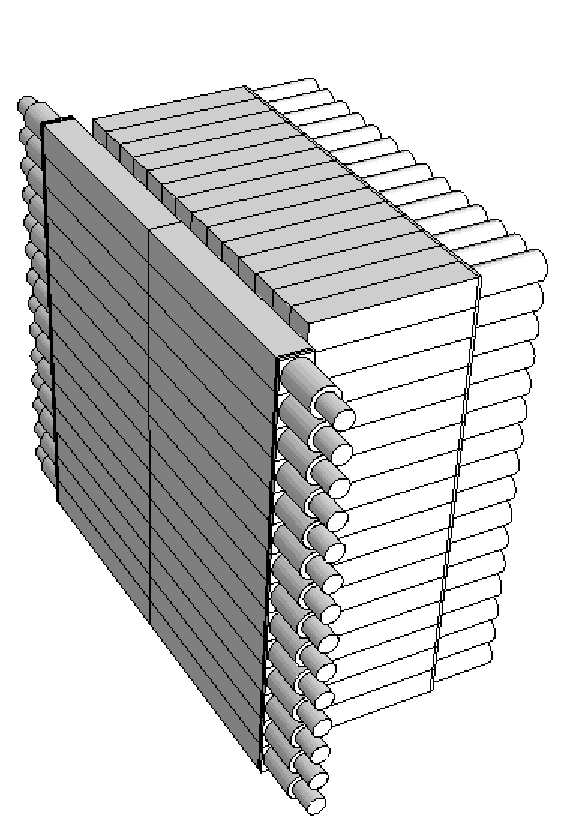
\includegraphics[width=0.5\textwidth]{shms_calo_sk.eps}\\
      }
    $2\times13$ blocks for preshower \\
    $14\times16$ blocks for shower
    \end{column}
  \end{columns}
\end{frame}

\begin{frame}{Calorimeter E/P}
  E/P peak should be at 1 for an electromagnetic shower
  \begin{figure}
    \centering
    \begin{minipage}[b]{0.4\textwidth}
      \includegraphics[width=\textwidth]{hms_eoverp.pdf}
      \caption{HMS Calorimeter E/P}
    \end{minipage}
  \hfill
  \begin{minipage}[b]{0.4\textwidth}
    \includegraphics[width=\textwidth]{shms_eoverp.pdf}
    \caption{SHMS Calorimeter E/P}
  \end{minipage}
\end{figure}{}
\end{frame}{}

\begin{frame}{Calibration formalism}{Definitions}
  \begin{columns}
    \begin{column}[T]{0.7\textwidth}
      \begin{block}{Block Energy}
        \smaller
        The observed energy in a calorimeter block is \\
        $ E_i = G_i A_i$\\
        where $G_i$ and $A_i$ are the gain constant and raw ADC value for the $i$th block, respectively.  
      \end{block}
      \begin{itemize}
        \item $n$ : number of pmts in calorimeter
        \item $N$ : number of events in calibration sample
        \item $E_i^{(k)}= G_i A_i^{(k)}$ : energy seen by $i$th pmt in $k$th event
        \item $\displaystyle E_k = \sum_i^n E_i^{(k)}$ : total energy in $k$th event
      \end{itemize}

      %PS: Preshower: 2*13, 
      %\texttt{\smaller adc is P.cal.pr.goodNeg(Pos)AdcPulseInt(1-13)}
      %Shower:14*16,
      %\texttt{ \smaller adc = P.cal.fly.goodAdcPulseInt(1-224)}

    \end{column}
    \begin{column}[T]{0.3\textwidth}
      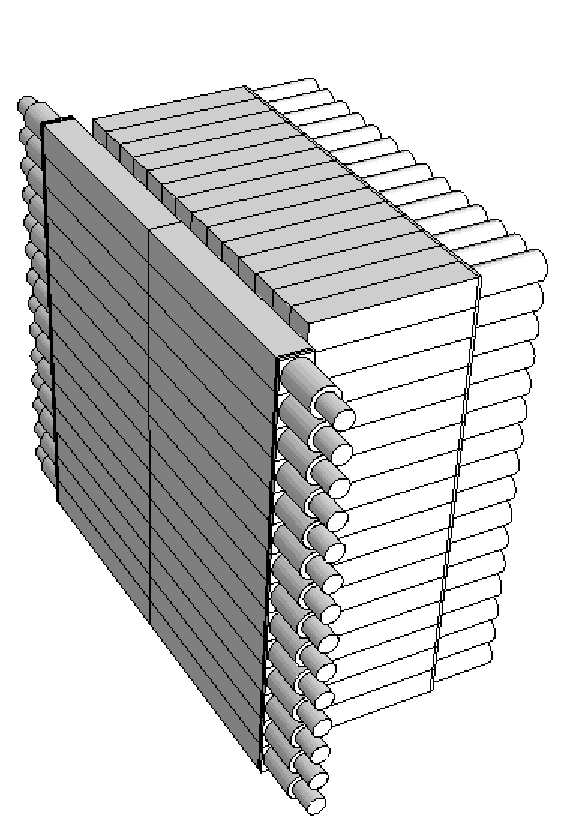
\includegraphics[width=0.9\textwidth]{shms_calo_sk.eps}
    \end{column}
\end{columns}
\end{frame}

\begin{frame}{Calorimeter Gain Constants}
  \centering
  \vspace{-0.5cm}
  \begin{columns}
    \begin{column}[T]{0.8\textwidth}
      \begin{block}{HMS : $4\times13\times2$ constants}
        \includegraphics[width=\textwidth]{hms_calparam.png}\\
      \end{block}
    \end{column}
    \begin{column}[T]{0.2\textwidth}
      \smaller 
      \vspace{1cm}
      Note HMS has zeroed gain constants on negative sides without PMTs
    \end{column}
  \end{columns}
  \begin{columns}
    \begin{column}[T]{0.8\textwidth}
      \begin{block}{SHMS : $2\times14 + 14\times16$ constants}
        \includegraphics[width=\textwidth]{shms_calparam.png}\\
      \end{block}
    \end{column}
    \begin{column}[T]{0.2\textwidth}
      \smaller 
      \vspace{1cm}
      \alert{\textbf{Note SHMS has zeroed gain constants for perfectly good blocks/PMTs!!!}}
    \end{column}
  \end{columns}
\end{frame}

\begin{frame}{Algorithm}
The gain constant for each block is determined by minimizing the $\chi^2$, which is defined as the squared difference between a know energy(track momentum for electron) to the measured energy in the calorimeter. 
\begin{itemize}
    \item $\chi^2=\sum_k^N(P^{(k)}-\sum_i^nG_iA_i^{(k)})^2=\sum_k^N((P^{(k)}^2)+(\sum_i^nG_iA_i^{(k)})^2-2P^{(k)}\sum_i^nG_iA_i^{(k)})$
     \item $\frac{\partial\chi^2}{\partial G_i}=0$
     \item $\sum_k^N2(\sum_i^nG_iA_i^{(k)})A_j^{(k)}-2P_k\sum_i^nG_iA_i^{(k)}=0$
     \item $\sum_k^N\sum_i^nG_iA_i^{(k)}A_j^{(k)}=\sum_k^NP_k\sum_i^nG_iA_i^{(k)}$
     \item $\mathcal{Q}G=\vec{q_e}$
     \item $Q_lm = \sum_i^NE_l^iA_m^i$
\end{itemize}
\begin{equation}
        \mathcal{Q}\vec{\alpha}=\vec{q_e}
\end{equation}{}

\end{frame}

\begin{frame}{Algorithm}{normalization errors/systematic error source}
\begin{columns}
\begin{column}{0.5\textwidth}
N data $\vec{q_e}$ with different standard deviation $\sigma$ and a common relative normalization error of $\epsilon$. mean value is not affected but standard derivation is. 
\end{column}
\end{columns}
\end{frame}{}
\begin{frame}{Calibration Formalism}{Currently used algorithm}
  \smaller
  \begin{columns}
    \begin{column}{0.5\textwidth}
      \begin{enumerate}
        \item Initialize all gain constant to be $ G_i = 1$
        \item Build vectors and matrix from event sample
      \end{enumerate}

      \begin{itemize}
        \item $\Bar{P} = \frac{1}{N}\sum^N_k P^{(k)}$
        \item $\vec{q} _e = q_{e,i}= \frac{1}{N}(\sum^N_k E_i^{(k)} P^{(k)})$
        \item $\vec{q}_0 = q_{0,i}= \frac{1}{N}(\sum^N_k E_i^{(k)})$
        \item 
          {\smaller
      \(
        \mathcal{Q}=\frac{1}{N} \sum^N_k
        \begin{bmatrix}
          E_1^2 &  E_1E_2 & \dots \\
          E_1E_2 &  E_2^2 & \dots \\
          \vdots & \ddots & \\
          E_1E_{n}&\dots &  E^2_{n}
        \end{bmatrix}^{(k)}
      \)
    }
      \end{itemize}
      \end{column}
    \begin{column}{0.5\textwidth}

      \[
        \mathcal{Q} \vec{\alpha} = \vec{q}_e
      \]
      Solve for $\vec{\alpha}$
      \[
        \Delta_E  = \Bar{P} - \vec{\alpha}\cdot \vec{q}_e
      \]

      \[
        \mathcal{Q} \vec{x} = \vec{q}_0
      \]
      Solve for $\vec{x}$

      \[
        t_2 = \vec{q_0}\cdot\vec{x}
      \]

      \[ 
        G^{\prime} = (\frac{\Delta_E}{t2}\vec{x}) + \vec{\alpha}
      \]


%      mq.falphaU = mq.fQ.fullPivHouseholderQr().solve(mq.fqe);
%
%      double t1 = mq.fe0 - mq.falphaU.dot(mq.fq0); // temporary variable.
%      
%      mq.fQiq0 = mq.fQ.fullPivLu().solve(mq.fq0);
%
%      double t2 = mq.fq0.dot(mq.fQiq0); // another temporary variable
%      //  cout << "t2 =" << t2 << endl;
%
%      mq.falphaC = (t1 / t2) * mq.fQiq0 + mq.falphaU; // the sought gain constants
%
      %\overleftrightarrow{Q}=\overrightarrow{q}_0^T\overrightarrow{q}_0
    \end{column}%
    %\begin{column}{0.5\textwidth}
    %  \begin{align*}
    %    \begin{split}
    %      \overleftrightarrow{Q}*\overrightarrow{\alpha_u} &= \overrightarrow{q_e} , \Rightarrow{\overrightarrow{\alpha_u}} , \\
    %      \Delta &= e_0-\overrightarrow{\alpha} _u*\overrightarrow{q} _0, \\
    %      \overleftrightarrow{Q}* \overrightarrow{x_2} &= \overrightarrow{q_0}, \Rightarrow{\overrightarrow{x_2}} \\
    %      t_2 &= \overrightarrow{q_0}*\overrightarrow{x_2}, \\
    %      \overrightarrow{\mathrm{G}^{\,\prime}} &= (\frac{t_1}{t_2})*\overrightarrow{x_2}+\overrightarrow{\alpha_u}
    %    \end{split}{}  
    %  \end{align*}{}
    %\end{column}
  \end{columns}
 
\end{frame}

\begin{frame}{Typical selection}
  \includegraphics[width = 0.5\textwidth]{run6490uncalib.png}
\end{frame}

\begin{frame}{Result after calibration}
  \includegraphics[width = 0.5\textwidth]{run6490aftercalib.png}
\end{frame}

\begin{frame}{gain constant analysis}
    \begin{columns}
    \begin{column}[T]{0.5\textwidth}
    \includegraphics[width = \textwidth]{cal_gain_8_11.pdf}
    \end{column}{}
    \begin{column}[T]{0.5\textwidth}
      gain constant for one block for several runs. Black points are gain constant for 8-11 block for that run, Red points are the runs which doesn't have enough events to calibrate(150 events). The line is the average of gain constants weighted by the number of events per run.  
    //
     We use the weighted average for the block instead of the value from single calibration, so that the gain constant would be the result of all existing calibrations with enough selected events. 
    \end{column}{}
    \end{columns}
    \end{frame}{}

\begin{frame}{}
  \centering 
  Backup
\end{frame}

\begin{frame}{}
  \centering
  \includegraphics[width=0.5\textwidth]{eoverpuncalib.png}\\
  in \texttt{input.dat}: set gaussian fit range. in \texttt{THcPShowerCalib.h}: set LoThr and HiThr
  \begin{block}{}
    \centering \includegraphics[width=0.8\textwidth]{threshold.png}
    \label{fig:my_label}
  \end{block}
\end{frame}

\begin{frame}
Use SHMS as example, some electrons are detected by SHMS, We know that electron peak should locate at 1, which means sum of energy measured by each pmt should be equal to momentum. 
\begin{equation}
    \sum^{252}_i E_i*\alpha_{ci} = E = P
\end{equation}{}    
i: Blocks

N: Number of events(tracks)

j: number of hits per events
\end{frame}



\begin{frame}{}

\end{frame}{}

\end{document}
 
